\documentclass[12pt]{article}
\usepackage{amsmath, amsfonts, amssymb}
\usepackage{graphicx}
\DeclareMathOperator*{\argmax}{arg\,max}
\DeclareMathOperator*{\argmin}{arg\,min}
\DeclareMathOperator{\diag}{diag}
\DeclareMathOperator{\rank}{rank}
\title{Regression Analysis}
\author{J\'{e}r\^{o}me Maye}
\date{\today}
\begin{document}
  \maketitle

  \section{Maximum Likelihood Formulation}

  Let us define a set of $n$ realizations
  $\{\mathbf{y}_i\}_{i=1}^n\in\mathbb{R}^d$ of an
  observable random variable $\mathbf{Y}$ such that

  \begin{equation}\label{eqn:gencondmodel}
    \begin{aligned}
      \boldsymbol{\epsilon}_i \sim f_{\boldsymbol{\Theta}}, i = 1\cdots n\\
      \mathbf{y}_i = g(\mathbf{X}) + \boldsymbol{\epsilon}_i, i=1\cdots n,
    \end{aligned}
  \end{equation}

  \noindent where $\mathbf{X}\in\mathbb{R}^k$ is a latent random variable,
  $g(\cdot)$ an arbitrary function of $\mathbf{X}$,
  $\{\boldsymbol{\epsilon}_i\}_{i=1}^n\in\mathbb{R}^d$ are i.i.d. random
  variates generated according to a parametric family of distributions
  characterized by the \emph{probability density function} (pdf)
  $f_{\boldsymbol{\Theta}}$.

  We can define the \emph{residuals} as

  \begin{equation}\label{eqn:residuals}
    \begin{aligned}
      \mathbf{e}_i = \mathbf{y}_i - g(\mathbf{X}),
    \end{aligned}
  \end{equation}

  \noindent which are therefore distributed according to 
  $f_{\boldsymbol{\Theta}}$.

  In order to estimate $\mathbf{X}$, one can use Maximum Likelihood Estimation
  (MLE) and derive the likelihood function of the residuals

  \begin{equation}\label{eqn:likelihoodfun}
    \begin{aligned}
      \mathcal{L}(\mathbf{X}\mid \mathbf{y}_1,\cdots,\mathbf{y}_n)
        \stackrel{\mathrm{i.i.d.}}{=}
        \prod_i^n f_{\boldsymbol{\Theta}}(\mathbf{e}_i;\mathbf{X}).
    \end{aligned}
  \end{equation}

  \noindent The sought estimate for $\mathbf{X}$ is then found by maximizing
  \eqref{eqn:likelihoodfun}

  \begin{equation}\label{eqn:maxlikelihood}
    \begin{aligned}
      \mathbf{\hat{X}} = \argmax_{\mathbf{X}}\mathcal{L}(\mathbf{X}
        \mid \mathbf{y}_1,\cdots,\mathbf{y}_n),
    \end{aligned}
  \end{equation}

  \noindent which, for the sake of simplicity, is turned into

  \begin{equation}\label{eqn:minllikelihood}
    \begin{aligned}
      \mathbf{\hat{X}} =
        \argmin_{\mathbf{X}}-\ln\mathcal{L}(\mathbf{X}\mid
        \mathbf{y}_1,\cdots,\mathbf{y}_n)=
        \sum_i^n -\ln(f_{\boldsymbol{\Theta}}(\mathbf{e}_i;\mathbf{X})).
    \end{aligned}
  \end{equation}

  \section{Normally Distributed Residuals}

  If we assume that
  $f_{\boldsymbol{\Theta}}=\mathcal{N}(\mathbf{0},\boldsymbol{\Sigma})$,
  where $\boldsymbol{\Sigma}$ is the covariance matrix of the residuals,
  \eqref{eqn:minllikelihood} becomes

  \begin{equation}\label{eqn:minllikelihoodnorm}
    \begin{aligned}
      \mathbf{\hat{X}} &=
        \argmin_{\mathbf{X}}\frac{n k}{2}\ln(2\pi)+
          \frac{n}{2}\ln(|\boldsymbol{\Sigma}|)+\frac{1}{2}
          \sum_{i=1}^n\mathbf{e}_i^T\boldsymbol{\Sigma}^{-1}\mathbf{e}_i
          \\&=\argmin_{\mathbf{X}}
          \sum_{i=1}^n\mathbf{e}_i^T\boldsymbol{\Sigma}^{-1}\mathbf{e}_i
          \\&=\argmin_{\mathbf{X}}
          \sum_{i=1}^n d_i^2,
    \end{aligned}
  \end{equation}

  \noindent where $d_i$ the Mahalanobis distance for error term $\mathbf{e}_i$.
  From \eqref{eqn:minllikelihoodnorm}, we can recognize the formulation of a
  \emph{least-squares} problem and therefore borrow its methods for solving it.
  We can also derive the different variants of least-squares problem from
  \eqref{eqn:minllikelihoodnorm}:

  \begin{itemize}
    \item \emph{Ordinary Least-Squares} (OLS): $d=1$ and
      $\boldsymbol{\Sigma}=\sigma^2\mathbf{1}$
    \item \emph{Weighted Least-Squares} (WLS):
      $\boldsymbol{\Sigma}=\diag([\sigma_1^2,\cdots,\sigma_d^2]^T)$
    \item \emph{Generalized Least-Squares} (GLS): full problem
  \end{itemize}

  \section{Robust Regression}

  The field of robust regression deals with outliers in the residuals
  distribution. A way to solve this issue is to use
  \emph{M-Estimators}. The principle is to define a residuals distribution that
  has heavier tails. The outliers will thus be more likely than with the normal
  distribution.

  An M-Estimator is defined using a so-called $\rho$-function or
  \emph{cost function} such that the pdf of the residuals is

  \begin{equation}\label{eqn:mestimatorpdf}
    \begin{aligned}
      f_{\boldsymbol{\Theta}}(\mathbf{e}_i) = \exp(-\rho(d_i)).
    \end{aligned}
  \end{equation}

  \noindent Therefore, \eqref{eqn:minllikelihood} becomes

  \begin{equation}\label{eqn:minllikelihoodmest}
    \begin{aligned}
      \mathbf{\hat{X}} &=
        \argmin_{\mathbf{X}}\sum_{i=1}^n \rho(d_i).
    \end{aligned}
  \end{equation}

  \noindent Additionally, the \emph{influence function}, denoted $\psi$, is
  defined as

  \begin{equation}\label{eqn:influence}
    \begin{aligned}
      \psi(x) \stackrel{\mathrm{def}}{=} \frac{\partial \rho}{\partial x} (x)
    \end{aligned}
  \end{equation}

  \noindent And finally, the \emph{weight function} $w$, also known as the
  attenuation function, is defined as

  \begin{equation}\label{eqn:weight}
    \begin{aligned}
      w(x) \stackrel{\mathrm{def}}{=} \frac{\psi(x)}{x}.
    \end{aligned}
  \end{equation}

  It can be demonstrated, through the chain rule of derivation, that
  \eqref{eqn:minllikelihoodmest} can be expressed as

  \begin{equation}\label{eqn:minllikelihoodmest2}
    \begin{aligned}
      \mathbf{\hat{X}} &=
        \argmin_{\mathbf{X}}\sum_{i=1}^n w(d_i)d_i^2,
    \end{aligned}
  \end{equation}

  \noindent which can be interpreted as an
  \emph{Iteratively Reweighted Least-Squares} (IRLS) problem. Furthermore, if
  $\rho(x)=x^2$, this corresponds to the standard least-squares problem.

  \subsection{Modified Blake-Zisserman M-Estimator}

     The modified Blake-Zisserman M-Estimator defines the $\rho$-function as

      \begin{equation}\label{eqn:bzrho}
        \begin{aligned}
          \rho(d_i) = -\ln(\exp(-d_i^2) + \varepsilon),
        \end{aligned}
      \end{equation}

      \noindent where $\varepsilon$ is a parameter. Note that underlying pdf
      is not a proper since it does not integrate to $1$. The cost function in
      \eqref{eqn:bzrho} approximates the standard
      least-squares cost function for inliers while it asymptotically tends
      to $-\log(\varepsilon)$ for outliers. The weight function is computed as

      \begin{equation}\label{eqn:bzw}
        \begin{aligned}
          w(d_i) = \frac{\exp(-d_i^2)}{\exp(-d_i^2) + \varepsilon}.
        \end{aligned}
      \end{equation}

      Our goal is to tailor $\varepsilon$ in such way that residuals considered
      as inliers receive a weight close to $1$ and outliers a weight close to
      $0$. We can first state the distribution of the squared Mahalanobis
      distances

      \begin{equation}\label{eqn:mddist}
        \begin{aligned}
          d_i^2 \sim \mathcal{X}^2_d,
        \end{aligned}
      \end{equation}

      \noindent which follows from the fact that the chi-squared distribution
      with $k$ degrees of freedom is the distribution of a sum of the squares of
      $k$ independent standard normal random variables. The cumulative
      distribution function (cdf) $F$ gives us the probability that a random
      variable takes a value less than or equal to another value. On the other
      hand, the inverse cdf (icdf) tells us this value for a given probability.
      This means that we can choose a probability threshold $p_t$ and query the
      squared Mahalanobis distance for which the samples have probability $p_t$
      of being less than or equal. Furthermore, we can set the weight $w_t$ that
      we want to assign at this threshold and solve \eqref{eqn:bzw} for
      $\varepsilon$

      \begin{equation}\label{eqn:epsilon}
        \begin{aligned}
          \varepsilon = \frac{1 - w_t}{w_t}\exp(-F^{-1}_d(p_t)).
        \end{aligned}
      \end{equation}

      Fig.~\ref{fig:bz3d} and \ref{fig:bz6d} illustrate these derivations for
      $d=3$ and $d=6$, $p_t=0.999$, and $w_t=0.1$.

      \begin{figure}[t]
        \centering
        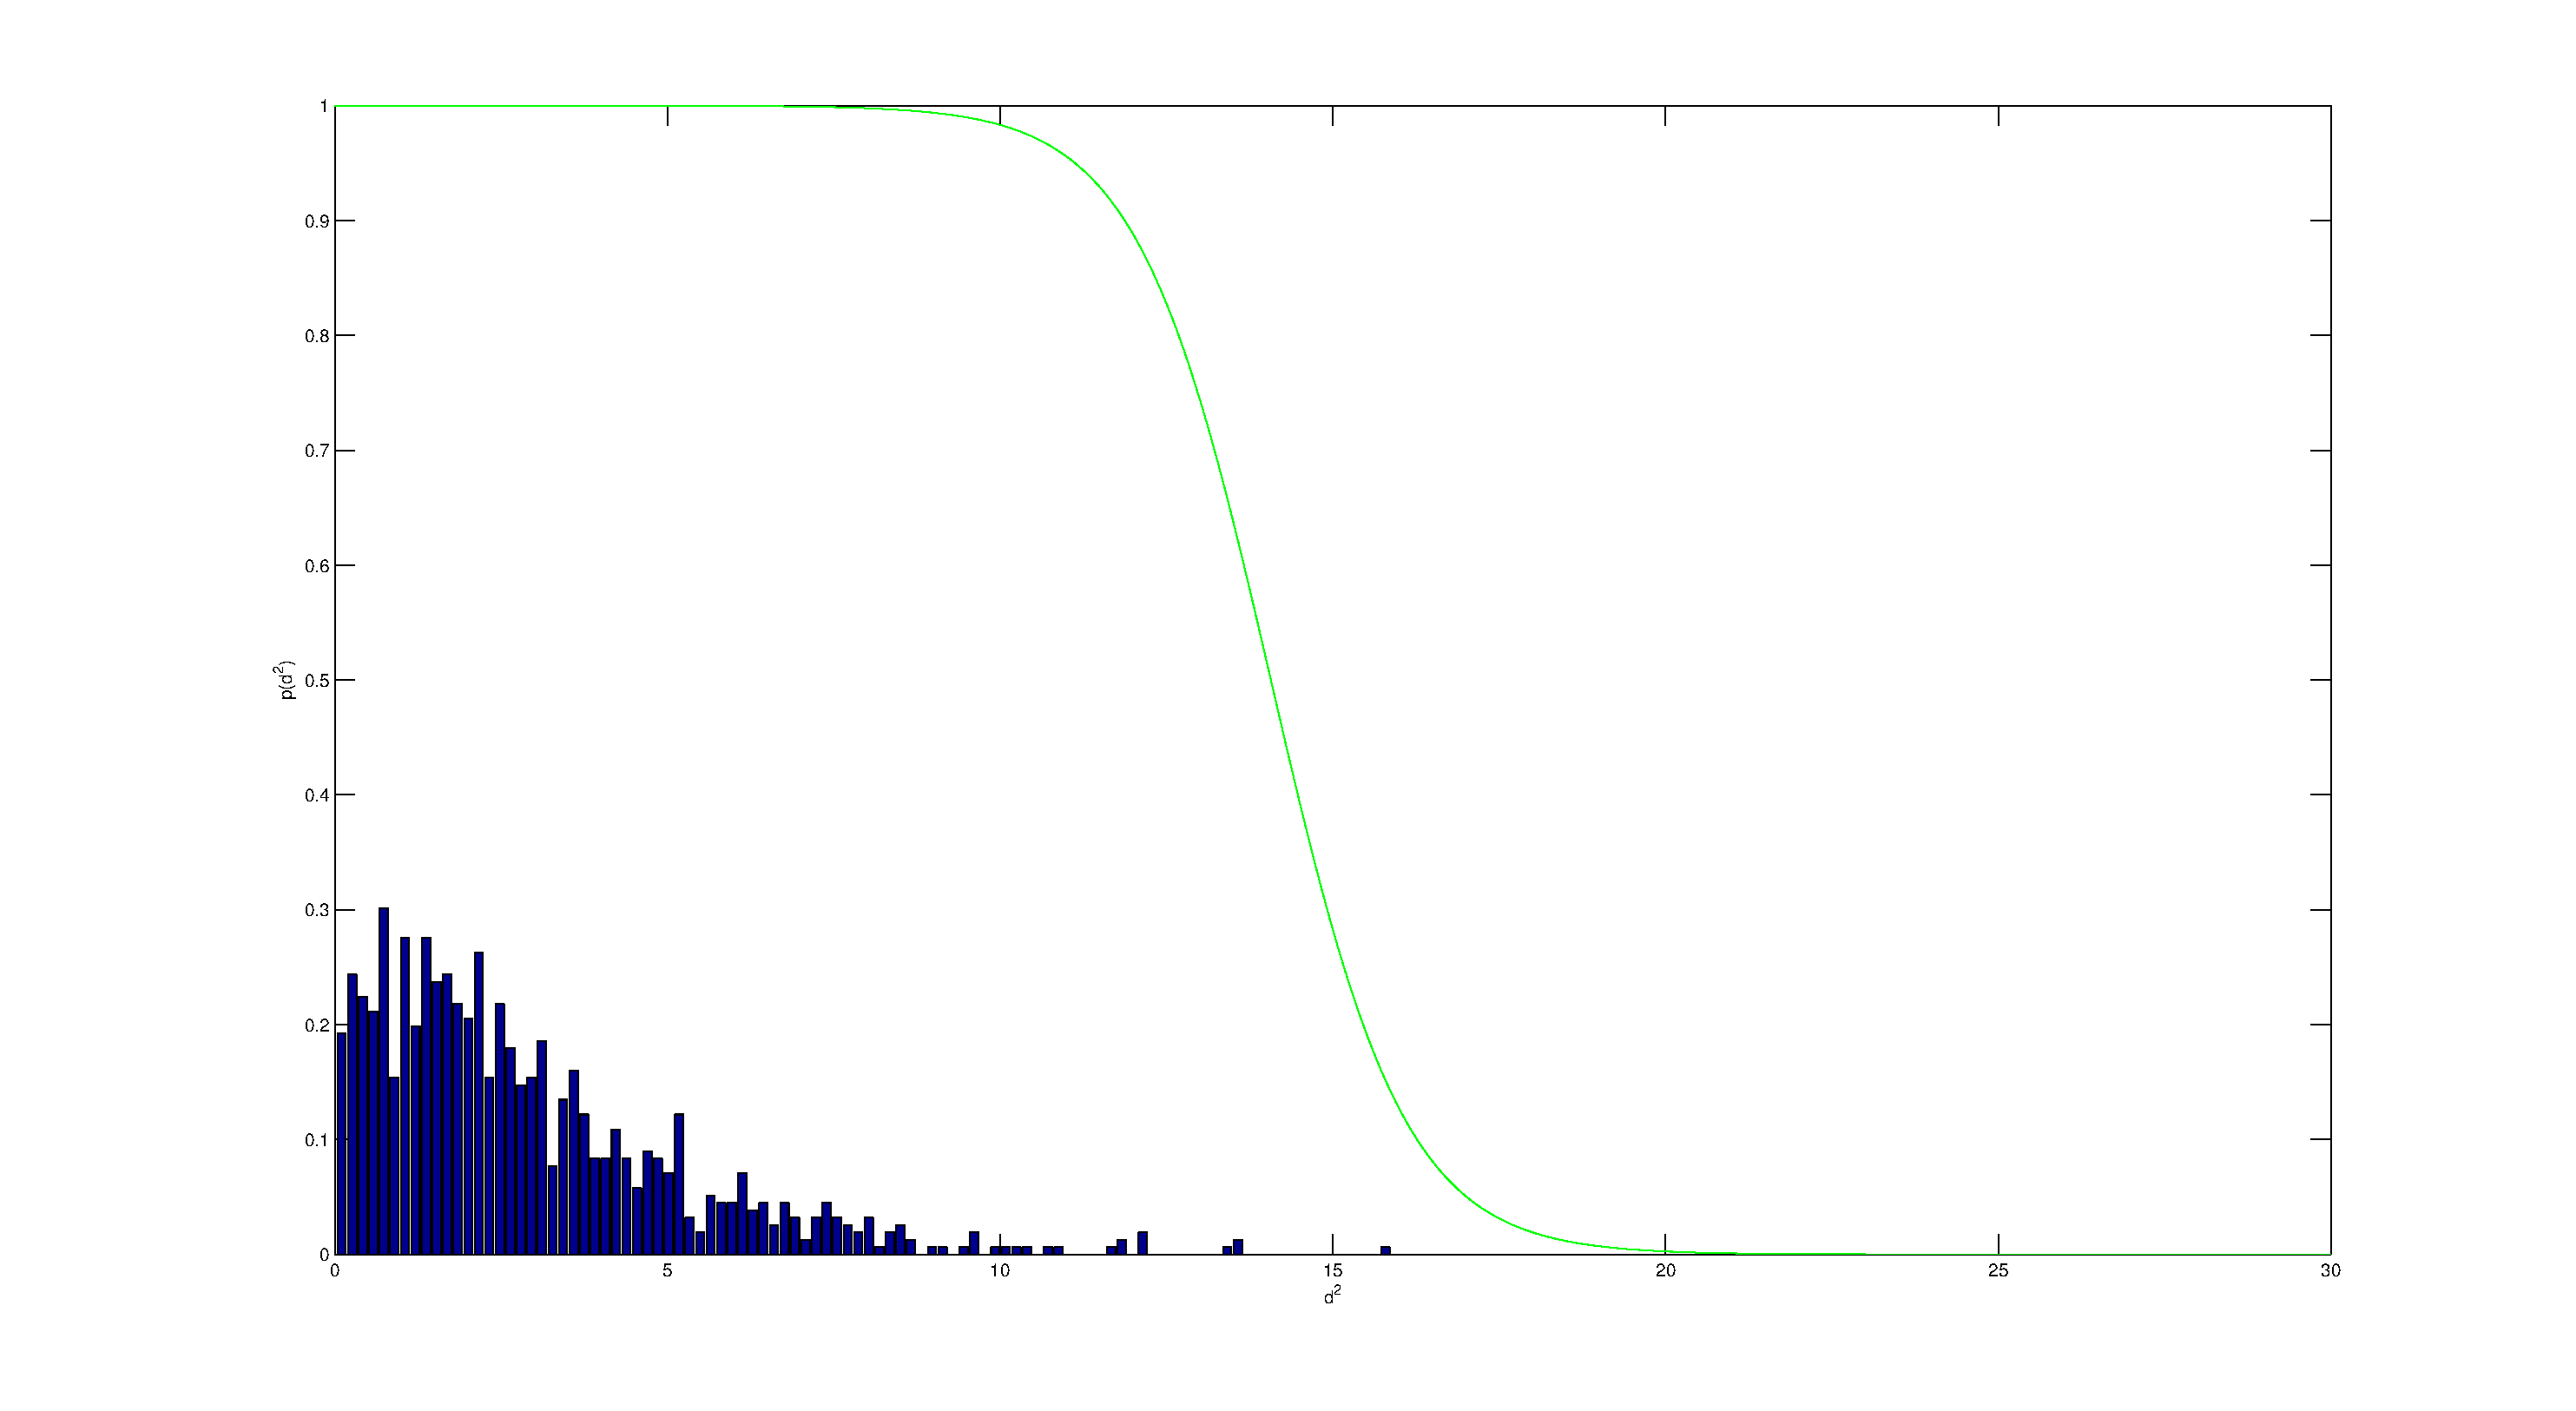
\includegraphics[scale = 0.3]{bz3d}
        \caption{Normalized histogram of 3D squared Mahalanobis distances and
          their corresponding weights with $p_t=0.999$ and $w_t=0.1$}
        \label{fig:bz3d}
      \end{figure}

      \begin{figure}[t]
        \centering
        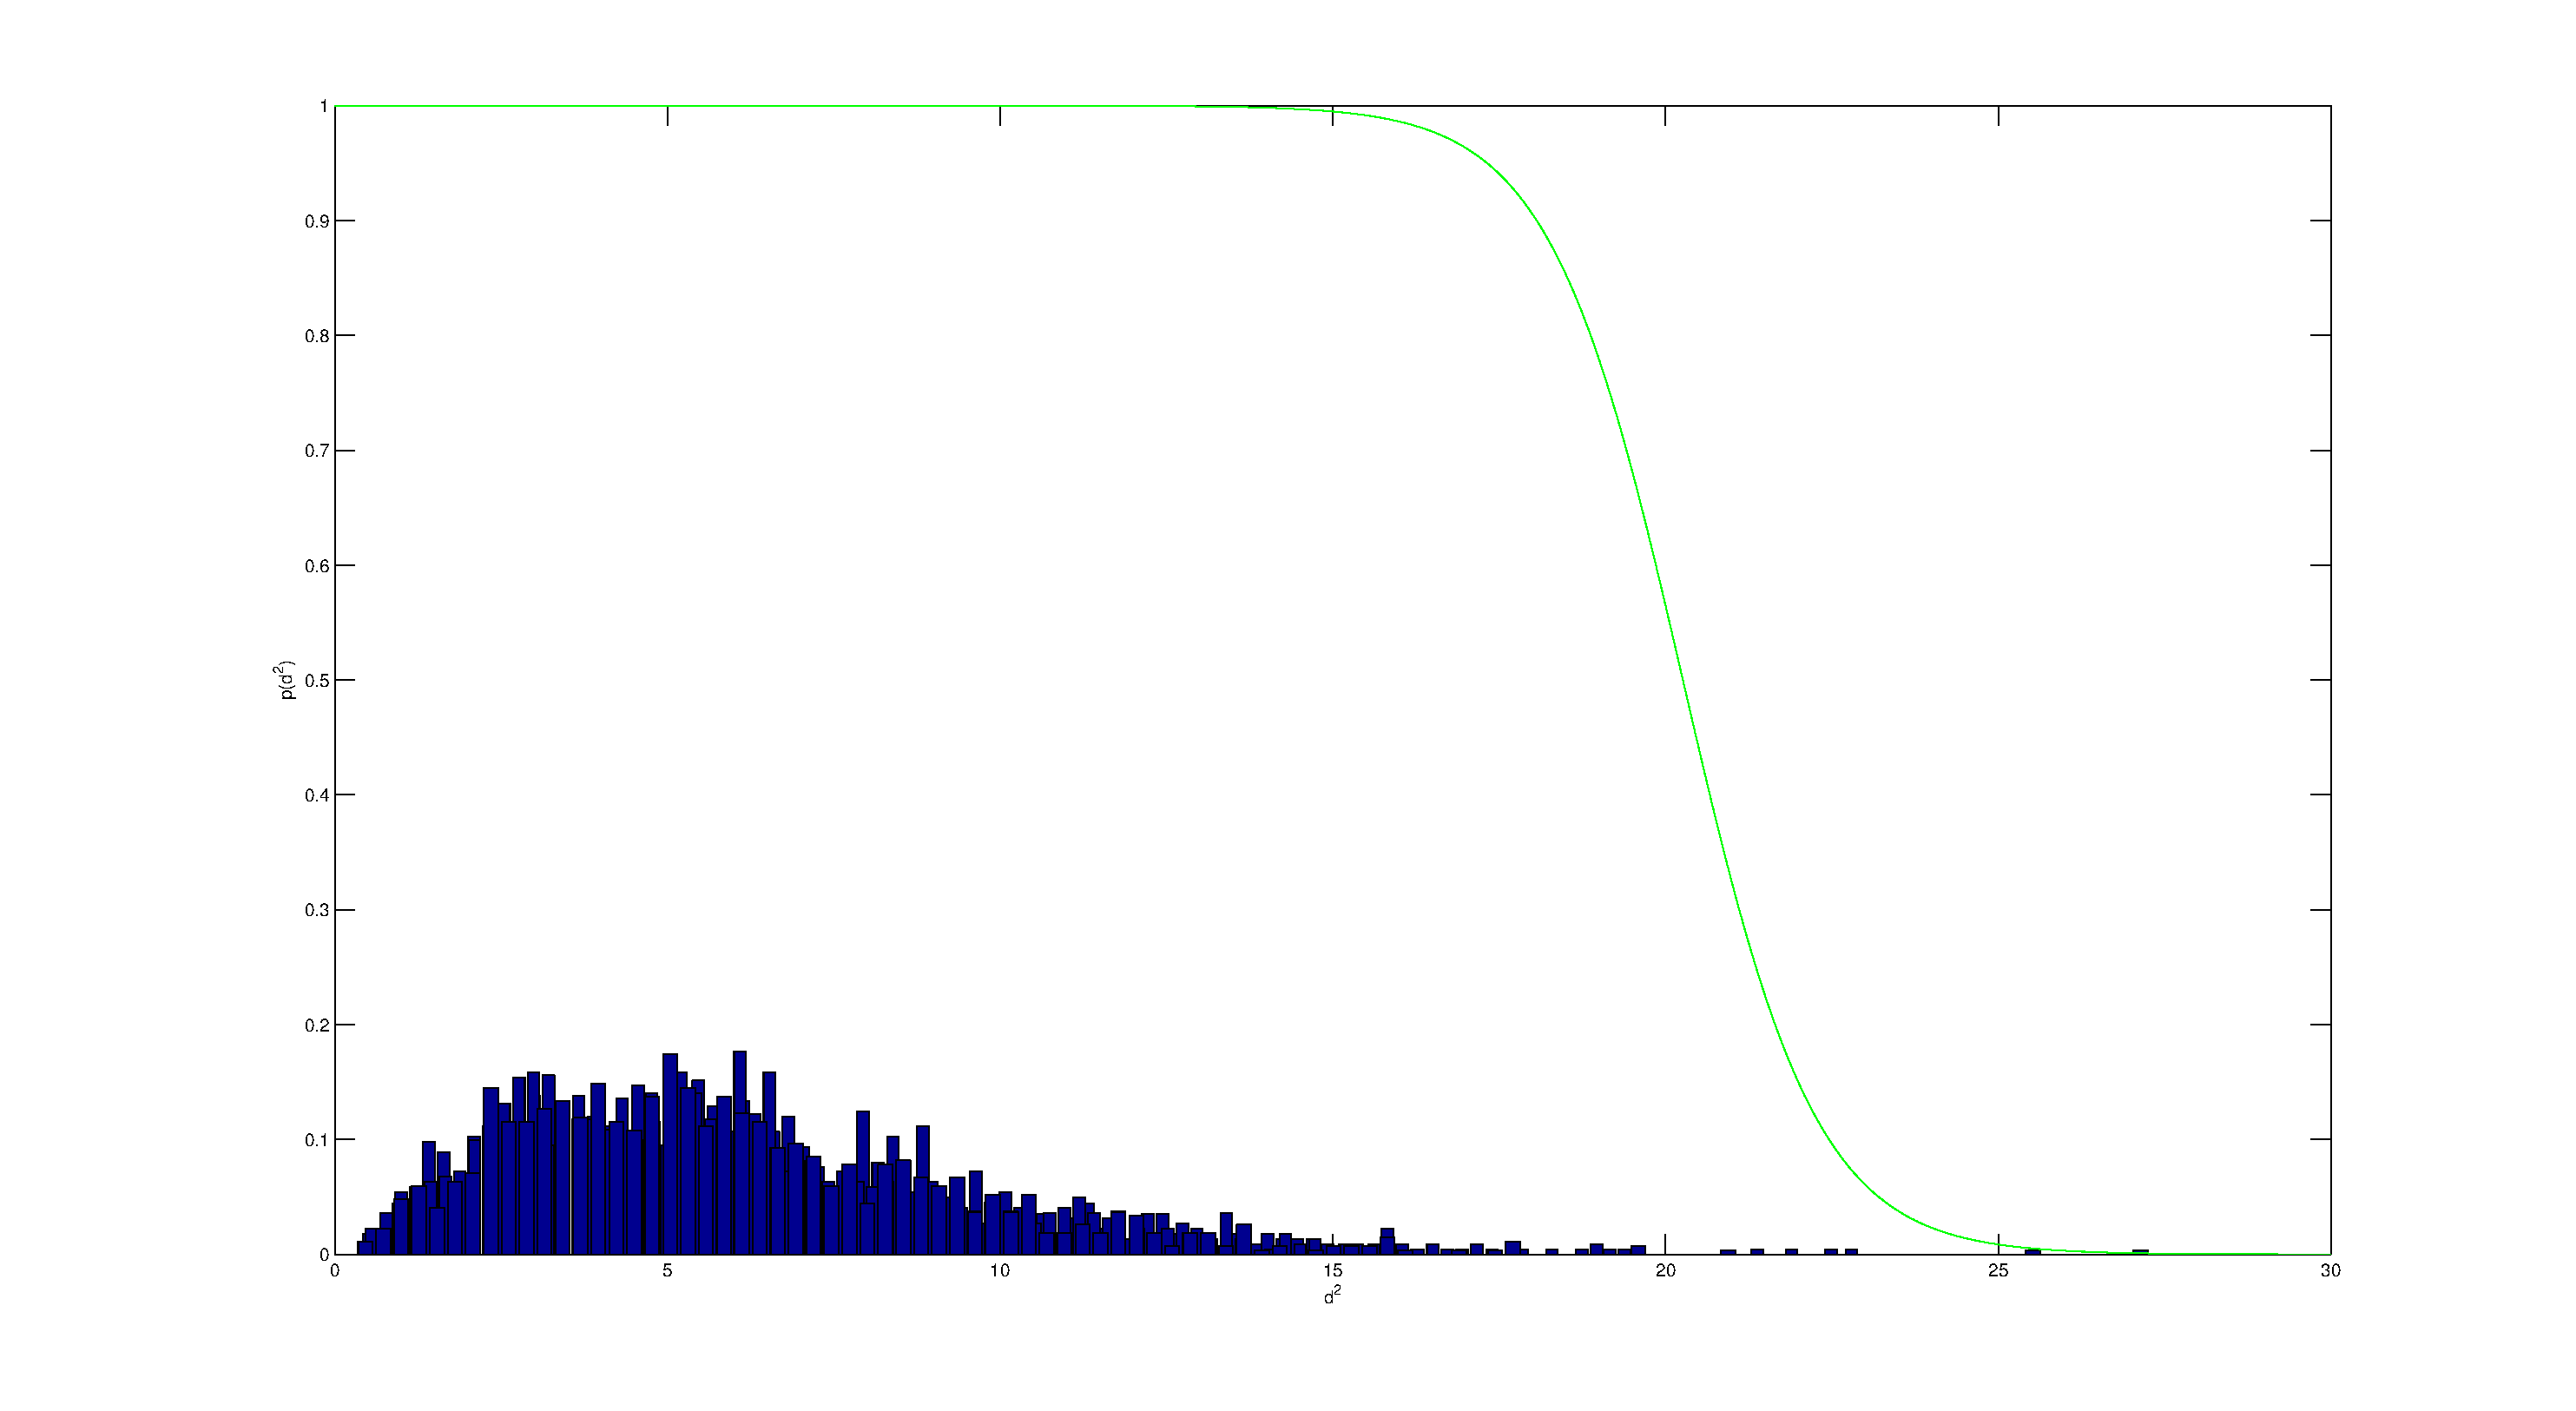
\includegraphics[scale = 0.3]{bz6d}
        \caption{Normalized histogram of 6D squared Mahalanobis distances and
          their corresponding weights with $p_t=0.999$ and $w_t=0.1$}
        \label{fig:bz6d}
      \end{figure}

\end{document}
